\section{Transfer of Thermal Energy}

%Conduction

%\subsection{Conduction of Heat by Different Materials}
%\begin{itemize}
%\item{Preparation Time: 2 minutes}
%\item{Materials: wooden stick, metal rod, candle, match}
%\item{Procedure: Light the candle and set the stick and rod to rest with one end in the flame (the stick should not light on fire if you just grabbed it from outside, but you can dampen it to be sure). Teach your lesson for a couple minutes and then check to see if it is ready. Have students touch the end (the end NOT in the flame) of each and determine which is hotter. The metal should be significantly warmer than the stick.}
%\item{Variation: Drip candle wax at even intervals along both the wooden stick and the metal rod. As heat is conducted along each, the wax will melt and drop off. You should see a significant difference between rate of melting of the stick and metal. You can also stick beans into the wax before it dries, to get a more dramatic effect when the wax melts.}
%\item{Theory: Heat is conducted through metal much more efficiently than through wood; therefore the end of the metal rod will become hotter faster than the stick. You should be able to feel it easily, and if the candle is hot enough the metal will be almost too hot to hold.}
%\end{itemize}


\subsection{Heat Conduction}

\subsubsection*{Learning Objectives}
\begin{itemize}
\item{To observe the progression of heat through a solid} 
\item{To differentiate between good and bad heat conductors} 
\item{To explain the progression of heat through solids in terms of the motion of molecules} 
\end{itemize}

\subsubsection*{Background Information}
Heat moves through solid bodies by conduction. Some solids are very good conductors of heat while others are not. Heat energy always moves from a hot body to a cold body, which it can do easily in a good conductor but not in a bad conductor. In this way, heat moves through an object from the hot end to the cold end.  

\subsubsection*{Materials}
iron nail, piece of glass, wooden stick, candle with a holder, matches, chair, books or other supports

\subsubsection*{Hazards and Safety}
\begin{itemize}
\item{The nail will become quite hot after being in the candle flame. It is best to wait a minute after removing the candle before you pick it up to clean it off.} 
\end{itemize}

\subsubsection*{Preparation Procedure}
\begin{enumerate}
\item{Collect all materials.} 
\item{Light the candle.} 
\item{Use the lit candle to drip wax at even intervals along the glass, iron and wood (about 1 cm apart).} 
\item{Set the iron nail, glass and stick on the edge of a chair so that one end of each sticks out at least 4 cm beyond the edge of the chair and converge at the same point. They should not be touching at any point.} 
\end{enumerate}

\begin{figure}
\begin{center}
\def\svgwidth{100pt}
\input{./img/heat-conduction.pdf_tex}
\caption{Heat Conduction in Different Materials}
\label{fig:heat-conduction}
\end{center}
\end{figure}

\subsubsection*{Activity Procedure}
\begin{enumerate}
\item{Make sure that the glass, nail and stick are secure on the chair and meet at one point beyond the edge of the chair.} 
\item{Place the candle under the three objects so that the flame just touches the end of each. Use books if necessary to prop up the candle.} 
\item{Wait and observe the rate at which the wax melts on each of the three objects.} 
\item{Have students find other objects which they want to test for heat conduction.} 
\end{enumerate}

\subsubsection*{Results and Conclusions}
It will be seen that the wax on the iron nail melts quickly, near the candle at first and then moving back along the nail. The wax on the glass, however, melts very slowly and does not progress very far while the wax on the stick does not melt at all.  
This shows that heat moves quickly through metal and slowly through wood and glass, or that metal is a good conductor and glass and wood are bad conductors.  

\subsubsection*{Clean Up Procedure}
\begin{enumerate}
\item{Blow out the candle.} 
\item{Clean the wax off of the three objects and return all materials to their proper places.} 
\end{enumerate}

\subsubsection*{Discussion Questions}
\begin{enumerate}
\item{On which object did the wax melt the fastest?}
\item{On which object did the wax melt the slowest?}
\item{Which object is a good conductor?}
\item{Which objects are bad conductors?}
\item{What causes the wax to melt?}
\item{How does heat move through the objects?}
\end{enumerate}

\subsubsection*{Notes}
Metal, a good conductor of electricity, is also a good conductor of heat. This is why we use metal cooking pots but we pick them up with fabric. Metal has many free electrons which carry energy easily through the metal, whether the energy is heat or electricity. Wood and glass, however, cannot transmit heat easily and so will burn or melt before heat is transmitted through the whole body. This is why we can hold firewood from one end while it burns at the other end.  
If you use plastic, be careful as it will melt quickly before the wax does. This shows it to be a very bad conductor and is a good demonstration, but it is also dangerous if it melts on your skin.  


\subsection{Hot Water Hold}
\begin{itemize}
\item{Preparation time: 10 minutes}
\item{Materials: 3 beakers or drinking glasses, a thermos of very hot water 3 metal coins, a piece of cloth, a piece of rubber strip}
\item{Procedure: Pour hot water into the three beakers. Ask for three students to help with the demonstration. One student will hold his glass using rubber strip to protect against the heat. One will use fabric. One will use metal coins. Tell the students they can put down their beaker if it becomes too hot.}
\item{Theory: Metal is a good conductor of heat, and so we expect that the student using metal coins will only be able to last a short time. rubber strip is a poor conductor of heat (a good insulator), and so will protect its student’s hands for a longer time. Thus, we expect the student using rubber strip to last a long time.}
\end{itemize}


\subsection{Copper Coil Candle Snuffer}
\begin{itemize}
\item{Preparation Time: 5 minutes}
\item{Materials: thick copper wire about 40 cm, candle, match}
\item{Procedure: Bend the copper wire into a spiral coil, leaving a length enough for a handle. It should be in the shape of a candle snuffer but clearly open. Light a candle and then put out the flame with your new snuffer.}
\item{Theory: Metal, especially copper, conducts heat readily. By putting the copper coil over a flame, you allow the copper to conduct all of the heat away from the flame, careful not to hurt your hand, depriving the flame of its own heat source.}
\end{itemize}


%Convection

%\subsection{Sawdust Water Currents}
%\begin{itemize}
%\item{Preparation Time: 1 minute}
%\item{Materials: sawdust, water, beaker, heat source}
%\item{Procedure: Fill the beaker with water and pour in a handful of sawdust so that the sawdust spreads out through the water. Heat the water over a candle or jiko and watch the sawdust cycle through the water from top to bottom.}
%\item{Theory: As water is heated, it moves up, displacing the cooler water above it. In this way, heated water continually cycles. As water heats, it moves up and cools, whereby it is later displaced by newly heated water moving up. The sawdust follows the currents in the water so you can clearly see the cycle.}
%\end{itemize}


\subsection{Convection}

\subsubsection*{Learning Objectives}
\begin{itemize}
\item{To observe convection currents in water}
\item{To explain the transfer of heat in fluids}
\end{itemize}

\subsubsection*{Background Information}
While solids transfer heat by conduction, liquids and gases transfer heat by convection.  In convection, energy is carried by molecules as they move through a liquid or gas, thereby transferring the heat from one place to another.

When a fluid is heated, the molecules with the most energy, namely the hot fluid, rises as its density decreases with temperature.  The cooler fluid, or molecules with less energy, move down to replace the warmer liquid.  By moving down, the cooler fluid then gains heat.  The warmer fluid which moved up loses its heat and moves down again.  This cycle repeats forever.  It is called a convection current.

We normally cannot see the convection currents in a fluid because the fluid is invisible or uniform.  However, if we put particles in the fluid so that they float in the middle, they will follow the convection currents.

\subsubsection*{Materials}
Water, clear water bottle, sawdust, source of heat

\subsubsection*{Hazards and Safety}
\begin{itemize}
\item{Do not hold the bottle too close to the heat source as it will melt.  The convection will work even if the heat is not strong.}
\end{itemize}

\subsubsection*{Preparation Procedure}
\begin{enumerate}
\item{Collect all materials.  Sawdust can be found at a carpenter's shop or can be made at home.  You want small pieces.}
\item{Fill the water bottle about 10 cm with water.}
\item{Pour some sawdust into the bottle so that it is visible in the water but does not absorb the water.}
\end{enumerate}

\subsubsection*{Activity Procedure}
\begin{enumerate}
\item{Turn on or light the heat source.}
\item{Hold the bottle with the water and sawdust above the heat so that the bottle receives heat but does not melt.}
\item{After a few minutes, observe the motion of the sawdust in the water.}
\end{enumerate}

\begin{figure}
\begin{center}
%\def\svgwidth{150pt}
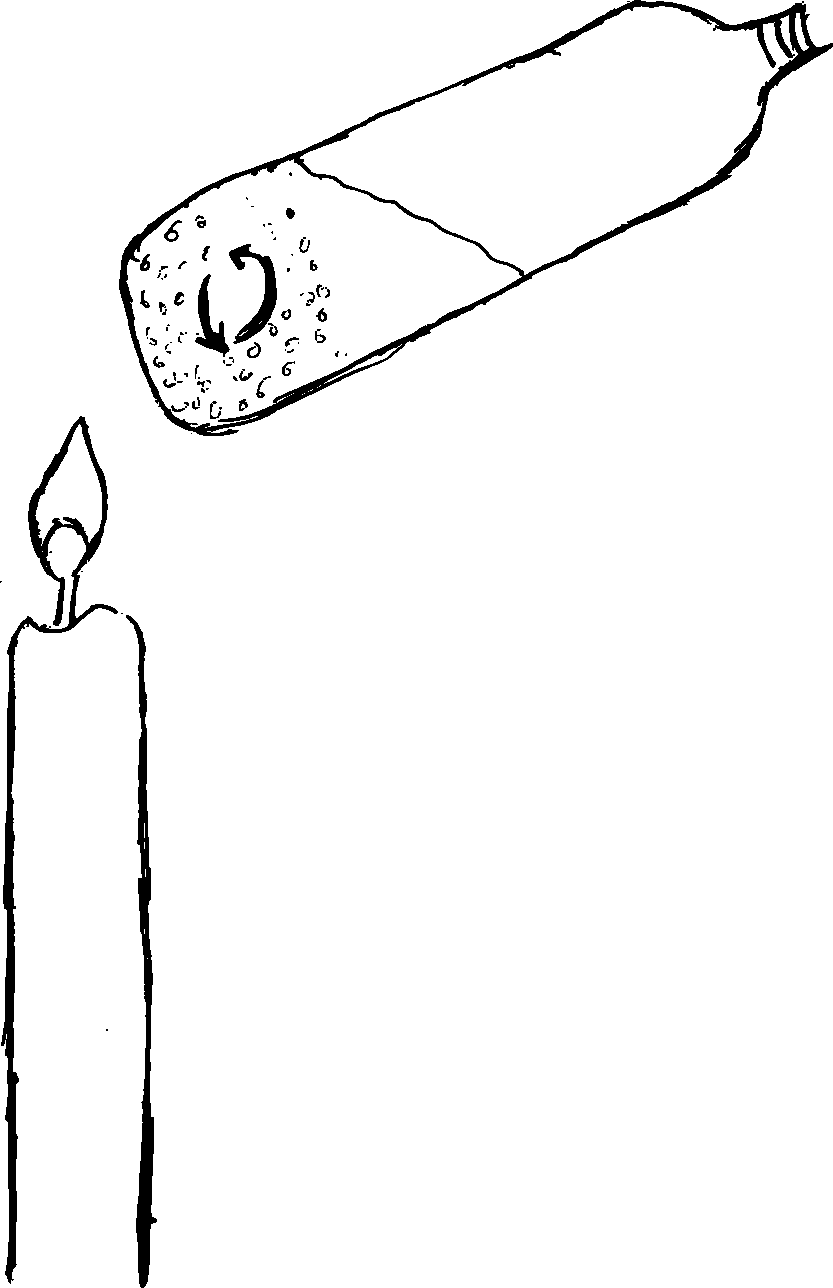
\includegraphics{./img/convection.png}
\caption{Thermal Convection}
\label{fig:convection}
\end{center}
\end{figure}

\subsubsection*{Results and Conclusions}
As the water in the bottle becomes warmer, the sawdust will be seen to move up.  After that it will begin to sink again.  This is because it is following the water in which it rests.  As the water at the bottom becomes warmer, it moves up.  At the top, there is less heat so the water cools again.  Then it sinks again to replace the new warm water rising again.  This cycle continues and causes the sawdust to continue circling from top to bottom and back.

\subsubsection*{Clean Up Procedure}
Dispose of the water and return all materials to their proper places.

\subsubsection*{Discussion Questions}
\begin{enumerate}
\item{Describe the motion of the sawdust.}
\item{Why does the sawdust move like this?}
\item{How is this type of heat transfer different from that in solids?}
\end{enumerate}

\subsubsection*{Notes}
Convection occurs in all gases and liquids.  The currents can be seen in many forms, like the movement and formation of clouds or the movement of smoke.


\subsection{Thermal Windmills}
\begin{itemize}
\item{Preparation Time: 1 minute}
\item{Materials: Windmills from another demo “Windmills,” candle, match}
\item{Procedure: If you have already created the windmill, set it up so that it spins horizontally about 10 cm above a candle. Light the candle and watch the windmill rotate.}
\item{Theory: As air is heated, it rises, displacing the cooler air above it. The heated air from the candle will force the windmill to rotate horizontally just as wind would cause it to rotate vertically.}
\end{itemize}


%Radiation

\subsection{Radiation}

\subsubsection*{Learning Objectives}
\begin{itemize}
\item{To explain the concept of radiation}
\item{To observe the heating effect of radiation}
\item{To explain the difference between reflection and absorption of heat}
\end{itemize}

\subsubsection*{Background Information}
Radiation is the transfer of heat through a vacuum.  It also occurs in air but it is difficult to detect because of the effect of convection.
However, the effects of radiation can be seen by observing the relative absorption and reflection of light and heat by various bodies.  A dark, rough surface will absorb heat while a shiny, smooth surface will reflect heat.  This is why many cars in hot places are painted white and why solar cookers are black.

\subsubsection*{Materials}
Two small pieces of flat wood, two metal plates, short candle, matches, small nails or glue, small kerosene burner or kibatari, steel wool

\subsubsection*{Hazards and Safety}
\begin{itemize}
\item{This activity should be done indoors to avoid any wind.}
\end{itemize}

\subsubsection*{Preparation Procedure}
\begin{enumerate}
\item{Cut the pieces of wood into equal sizes about 4 cm by 6 cm.  The exact size and shape is not important.}
\item{Cut two metal plates of equal size.  The metal around the outside of a D-cell battery is best.}
\item{Use the steel wool to rub the metal plates until they are clean and shiny.}
\item{Fix the metal plates to the pieces of wood so that the plates stand upright and the wood lies flat.  You can use glue or nails for this.}
\item{Light the kibatari.}
\item{Hold one of the metal plates above the kibatari until the plate's face is entirely coated in soot.  You should now have two upright metal plates: one black and one silver.}
\end{enumerate}

\begin{figure}
\begin{center}
%\def\svgwidth{200pt}
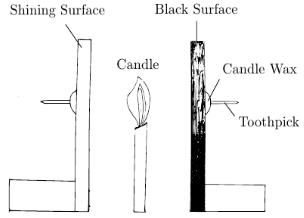
\includegraphics{./img/radiation.png}
\caption{Demonstration of the effect of surface colour on radiative heat transfer}
\label{fig:radiation}
\end{center}
\end{figure}

\subsubsection*{Activity Procedure}
\begin{enumerate}
\item{Light the candle.}
\item{On the back top of each of the metal plates, drip some wax from the candle.}
\item{Fix the used matches into the the wax so that they stick out horizontally from the back of the metal plate when the wax dries.}
\item{Place the candle on the table so that the flame is at the same height as the middle of each plate.}
\item{Place the metal plates a few inches to either side of the candle flame, facing in.}
\item{Wait and observe any changes.}
\end{enumerate}

\subsubsection*{Results and Conclusions}
The wax on the back of the black plate melts quickly and slides down the plate, bringing the match with it.  The wax on the silver plate takes a long time to melt.  This is because the black plate tends to absorb radiation while the silver plate tends to reflect radiation.  This causes the black plate's temperature to increase quickly, melting the wax.

\subsubsection*{Clean Up Procedure}
\begin{enumerate}
\item{Blow out the candle.}
\item{Return all materials to their proper places.}
\end{enumerate}

\subsubsection*{Discussion Questions}
\begin{enumerate}
\item{What happened to the wax on the back of the black plate?}
\item{What happened to the wax on the back of the silver plate?}
\item{Explain why the wax behaves differently on the black plate than on the silver plate.}
\end{enumerate}

\subsubsection*{Notes}
Two forms of heat transfer are present here: convection in the air and radiation.  However, the convection in the air carries heat equally to the black plate and silver plate.  The difference in heating rate is caused by the absorption rates.  Black materials absorb light and therefore heat, while shiny materials reflect light and therefore stay cool.
